\documentclass[a4paper,french,bookmarks]{article}

\usepackage{./Structure/4PE18TEXTB}

\newboxans
\usepackage{booktabs}

\begin{document}

    \renewcommand{\thesection}{\Roman{section}} 
    \renewcommand{\thesubsection}{\thesection.\Alph{subsection}}
    \setlist[enumerate]{font=\color{white5!60!black}\bfseries\sffamily}
    \renewcommand{\labelenumi}{\thesection.\arabic{enumi}.}
    \renewcommand*{\labelenumii}{\alph{enumii}.}
    \renewcommand*{\labelenumiii}{\alph{enumiii}.}
    
    \newcommand{\ON}{\mathbf{ON}}
    
    \stylizeDocSpe{Physique}{Devoir maison n° 9}{Fibre optique}{Pour le mardi 3 janvier 2023}
    
    \emph{Les fibres optiques sont de plus en plus utilisées dans le domaine des télécommunications. Elles permettent en effet des transmissions à grande distance. Après une étude générale des fibres à saut d'indice, puis une mise en équation simplifiée des modes de propagation, deux sources de limitation dans l'utilisation des fibres sont successivement analysées : la dispersion et l'atténuation.}\medskip
    
    Considérons une fibre optique dont le c\oe{}ur est un cylindre circulaire d'axe $\p{Oz}$, de rayon $R_1$ et d'indice optique $n_1$. Le point $O$ est le centre de la face d'entrée de la fibre. La gaine est également d'axe $\p{Oz}$, d'indice $n_2$, de rayon intérieur $R_1$ et de rayon extérieur $R_2$. Les indices vérifient l'inégalité $n_1 > n_2$. Une telle fibre est dite à saut d'indice.\medskip
    
    On considère un rayon lumineux arrivant en $O$ à l'entrée du c\oe{}ur de la fibre. Dans l'air, il est incliné d'un angle $\theta_0$ par rapport à l'axe $\p{Oz}$. Après réfraction dans le c\oe{}ur de la fibre, le rayon arrive à l'interface entre le c\oe{}ur et la gaine, avec un angle d'incidence $i_1$ par rapport à la normale au dioptre formé par le c\oe{}ur et la gaine.\medskip
    
    Tous les angles intervenant sont compris entre $0$ et $\frac{\pi}{2}$. L'indice de l'air est pris égal à $n_\text{air} = \qty{1,0}{}$. On pourra se référer à la figure \ref{fig:fig1} ci-dessous, réalisée dans le plan d'incidence, qui est un plan de symétrie pour la fibre.
    
    \begin{center}
        \begin{minipage}{0.8\linewidth}
            \centering
            \resizebox{\linewidth}{!}{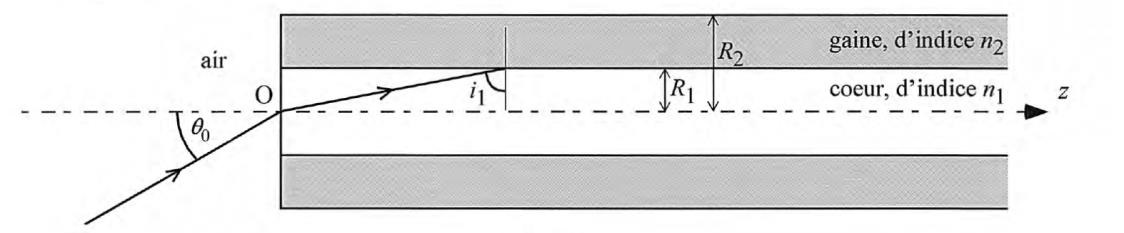
\includegraphics[]{dm9fig/dm9fig1.jpg}}
        \end{minipage}
        %
        %
        \text{}\\[2pt]
        %
        \begin{minipage}{0.9\linewidth}
            \captionof{figure}{Fibre optique à saut d'indice}
	        \label{fig:fig1}
        \end{minipage}
    \end{center}
    
    \section{Notions d'ouverture numérique et de mode}
    
    \begin{enumerate}
        \item Établir une relation entre les angles $i_1$, $\theta_0$ et les indices des milieux.
        
        \noafter
        %
        \boxans{
            D'après la loi de \textsc{Snell-Descartes}, on a $n_\text{air}\sin \theta_0 = n_1\sin{\frac{\pi}{2} - i_1}$, c'est-à-dire 
        }
        %
        \nobefore\yesafter
        %
        \boxansconc{
            \[ \cos i_1 = \dfrac{n_\text{air}}{n_1}\sin \theta_0\]
        }
        %
        \yesbefore
        
        \item Quelle est la condition portant sur $\sin i_1$ et les indices des milieux pour qu'il y ait réflexion totale à l'interface entre le c\oe{}ur et la gaine ?
        
        \noafter
        %
        \boxans{
            Soit $i_2$ l'angle d'un potentiel rayon réfracté à l'interface entre le c\oe{}ur et la gaine, de sorte que $n_1\sin i_1 = n_2\sin i_2$. On veut qu'il n'y ait pas réfraction, donc que $i_2 > \dfrac{\pi}{2}$. Par décroissance de $\sin$ sur $\into{\dfrac{\pi}{2}, \dfrac{3\pi}{2}}$, on a donc $\sin i_2 < 1$.
        }
        %
        \nobefore\yesafter
        %
        \boxansconc{
            On veut donc que $\sin i_1 < \dfrac{n_2}{n_1}$.
        }
        %
        \yesbefore
        
        \item On appelle \emph{ouverture numérique} de la fibre la quantité $\ON = \sqrt{{n_1}^2 - {n_2}^2}$. Quelle est, en fonction de $\ON$, la valeur maximale $\theta_{0, \text{max}}$ de l'angle $\theta_0$ au-delà de laquelle il n'y a plus réflexion totale à l'interface c\oe{}ur-gaine ? Calculer numériquement $\theta_{0, \text{max}}$ pour $n_1 = \qty{1.48}{}$ et $n_2 = \qty{1.46}{}$.
        
        \noafter
        %
        \boxans{
            On a $\sin^2 i_1 = 1 - \cos^2 i_1 = 1 - \dfrac{n_\text{air}^2}{{n_1}^2}\sin^2 \theta_0$ donc par croissance de la fonction carré sur $\bdR_+$, on a :
            %
            \[ 1 - \dfrac{n_\text{air}^2}{{n_1}^2}\sin^2 \theta_0 < \dfrac{{n_2}^2}{{n_1}^2} \qquad\text{donc}\qquad \dfrac{n_\text{air}^2}{{n_1}^2}\sin^2 \theta_0 < \dfrac{{n_1}^2 - {n_2}^2}{{n_1}^2} \qquad\text{donc}\qquad n_\text{air}\sin \theta_0 < \sqrt{{n_1}^2 - {n_2}^2} = \ON \]
        }
        %
        \nobefore\yesafter
        %
        \boxansconc{
            Par croissance de $\arcsin$, on a donc $\theta_{0, \text{max}} = \arcsin{\dfrac{\ON}{n_\text{air}}} = \arcsin{\ON}$.
            
            L'application numérique livre $\theta_{0, \text{max}} = \qty{0.43}{rad}$.
        }
        %
        \yesbefore
    \end{enumerate}
    
    La détermination des différents modes de propagation des ondes électromagnétiques dans une fibre optique fait appel aux équations de \textsc{Maxwell} et aux équations de propagation qui en découlent. Les solutions rigoureuses s'écrivent au moyen des fonctions de \textsc{Bessel}. Il est toutefois possible d'obtenir des solutions approchées, et d'appréhender la notion de modes avec un formalisme allégé, en s'appuyant sur des considérations simples d'optique ondulatoire.\medskip
    
    Considérons un plan de symétrie de la fibre contenant l'axe $\p{Oz}$. Soient deux rayons lumineux se propageant dans ce plan, au sein du c\oe{}ur de la fibre optique, l'un repéré par une simple flèche et l'autre par une double flèche. Les ondes associées à ces deux rayons sont supposées monochromatiques, cohérentes, et de longueur d'onde dans le vide $\lambda$. Elles subissent des réflexions totales entre le c\oe{}ur et la gaine, c'est-à-dire aux points $A_1, A_2, A_3, \dots$ pour le rayon repéré par une simple flèche, et aux points $B_1, B_2, B_3, \dots$ pour le rayon repéré par une double flèche. On note $\beta$ l'angle d'inclinaison de chacune des portions rectilignes de ces rayons par rapport à l'axe $\p{Oz}$ de la fibre.\medskip
    
    Soient $C$ et $D$ deux points des rayons $A_1A_2$ et $B_2B_3$ se trouvant dans un même plan orthogonal aux deux rayons. On considère également $E$ et $F$ deux points des rayons $B_2B_3$ et $A_3A_4$ se trouvant dans un même plan orthogonal aux deux rayons. La situation est représentée sur la figure \ref{fig:fig2} ci-dessous.
    
    \begin{center}
        \begin{minipage}{0.8\linewidth}
            \centering
            \resizebox{\linewidth}{!}{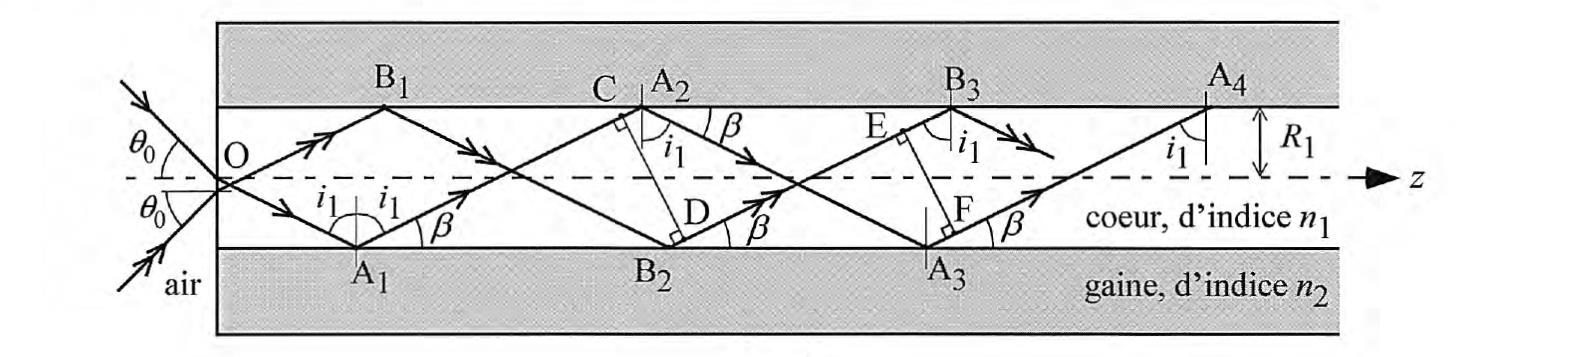
\includegraphics[]{dm9fig/dm9fig2.jpg}}
        \end{minipage}
        %
        %
        \text{}\\[2pt]
        %
        \begin{minipage}{0.9\linewidth}
            \captionof{figure}{Trajectoire des deux rayons}
	        \label{fig:fig2}
        \end{minipage}
    \end{center}
    
    \begin{enumerate}[resume]
        \item Dans un premier temps, on ne prend pas en compte les éventuels déphasages dus aux réflexions. En utilisant les points apparaissant sur la figure \ref{fig:fig2}, exprimer la différence de chemin optique $\delta$ entre les deux rayons allant du plan contenant $C$ et $D$ au plan contenant $E$ et $F$. La différence sera choisie de sorte que $\delta$ soit positif.
        
        \noafter
        %
        \boxans{
            On a en fait de multiple choix pour $C$ et $D$. Puisque les deux points restent dans le même plan, la différence de marche n'en est cependant pas affectée : on \guill{ajoute} ou \guill{retire} le même chemin aux deux rayons. C'est également le cas pour les points $E$ et $F$. On prendra donc $C = A_2$ et $F = A_3$. 
            
            Pour le rayon repéré par une simple flèche, on a le chemin $CF = \dfrac{2R_1}{\sin \beta}$.
            
            Pour obtenir la distance $DE$, on considère la distance horizontale entre $A_2$ et $A_3$ : on a $A_2A_3 = \dfrac{2R_1}{\cos \theta}$. On considère également la distance horizontale entre $C$ et $D$
        }
    \end{enumerate}
    
\end{document}